% Informe del Taller 3. Compilar con:  make informe   (tectonic, plantilla UD)
% Las cifras (\cifra...) y las tablas salen de desarrollo/exportar_informe.py: no se copian a mano.
\documentclass[11pt,letterpaper]{article}
\usepackage{ud-informe}
% Acento azul: el logo del programa (MCIC) es azul, así que se usa la gama azur del manual de marca en lugar del rojo.
% Para volver al rojo institucional de la plantilla, borrar estas dos líneas.
\colorlet{udrojo}{udazul}
\definecolor{udrojoosc}{HTML}{0C6F96}
% Generado por desarrollo/exportar_informe.py: NO editar a mano.
\newcommand{\cifraaugLoteVal}{0,00}
\newcommand{\cifraaugLoteValGana}{1}
\newcommand{\cifraaugLoteTe}{$-$0,33}
\newcommand{\cifraaugLoteTeGana}{1}
\newcommand{\cifraaugMuestraVal}{0,12}
\newcommand{\cifraaugMuestraValGana}{3}
\newcommand{\cifraaugMuestraTe}{$-$0,25}
\newcommand{\cifraaugMuestraTeGana}{1}
\newcommand{\cifraaugN}{5}
\newcommand{\cifralargoValDif}{$-$0,15}
\newcommand{\cifralargoTeDif}{$-$0,19}
\newcommand{\cifralargoBrechaSin}{1,09}
\newcommand{\cifralargoBrechaCon}{0,40}
\newcommand{\cifraablBnTe}{0,54}
\newcommand{\cifraablBnVal}{0,32}
\newcommand{\cifraablBnBrecha}{0,83}
\newcommand{\cifraablDropTe}{$-$0,52}
\newcommand{\cifraablDropVal}{$-$0,47}
\newcommand{\cifraablDropBrecha}{1,45}
\newcommand{\cifraablAmbosTe}{0,46}
\newcommand{\cifraablAmbosVal}{0,11}
\newcommand{\cifraablAmbosBrecha}{1,46}
\newcommand{\cifraablTresTe}{2,11}
\newcommand{\cifraablTresVal}{1,07}
\newcommand{\cifraablTresBrecha}{0,89}
\newcommand{\cifraablBrechaCompleta}{0,90}
\newcommand{\ciframlpTe}{88,44}
\newcommand{\cifracnnDocTe}{91,20}
\newcommand{\cifracnnPropTe}{92,10}
\newcommand{\cifracnnPropVsMlp}{3,66}
\newcommand{\cifracnnPropVsDoc}{0,90}
\newcommand{\cifradsMNISTTe}{98,80}
\newcommand{\cifradsMNISTVal}{98,72}
\newcommand{\cifradsMNISTGap}{$-$0,1}
\newcommand{\cifradsMNISTPeor}{97,2}
\newcommand{\cifradsMNISTBajo}{0,0}
\newcommand{\cifradsFashionMNISTTe}{90,27}
\newcommand{\cifradsFashionMNISTVal}{90,34}
\newcommand{\cifradsFashionMNISTGap}{0,1}
\newcommand{\cifradsFashionMNISTPeor}{72,2}
\newcommand{\cifradsFashionMNISTBajo}{4,3}
\newcommand{\cifradsKMNISTTe}{92,10}
\newcommand{\cifradsKMNISTVal}{97,15}
\newcommand{\cifradsKMNISTGap}{5,1}
\newcommand{\cifradsKMNISTPeor}{86,3}
\newcommand{\cifradsKMNISTBajo}{2,0}
\newcommand{\cifralrUno}{82,46}
\newcommand{\cifralrSinBnUno}{9,76}
\newcommand{\cifralrDos}{96,70}
\newcommand{\cifralrSinBnDos}{92,62}
\newcommand{\cifralrTres}{96,30}
\newcommand{\cifralrSinBnTres}{96,52}
\newcommand{\cifralrCuatro}{92,38}
\newcommand{\cifralrCinco}{76,30}
\newcommand{\cifraaccTest}{91,85}
\newcommand{\cifraaccVal}{97,40}
\newcommand{\cifraaccTr}{96,31}
\newcommand{\cifraerrTest}{815}
\newcommand{\cifralossIni}{0,374}
\newcommand{\cifralossFin}{0,117}
\newcommand{\cifraepocas}{5}
\newcommand{\cifraparA}{su}
\newcommand{\cifraparB}{tsu}
\newcommand{\cifraparN}{60}
\newcommand{\cifraparInv}{21}
\newcommand{\cifraclaseMejor}{tsu}
\newcommand{\cifraclaseMejorAcc}{96,5}
\newcommand{\cifraclasePeor}{su}
\newcommand{\cifraclasePeorAcc}{82,2}
\newcommand{\cifrabrechaValTest}{5,5}


\renewcommand{\UDtitulo}{Reconocimiento de caracteres \textit{kuzushiji} con redes convolucionales}
\renewcommand{\UDsubtitulo}{Aprendizaje profundo con PyTorch sobre KMNIST: núcleo del taller y extras}
\renewcommand{\UDtipo}{Taller 3}
\renewcommand{\UDasignatura}{Inteligencia Computacional Aplicada}
\renewcommand{\UDdocente}{Cesar Andrey Perdomo Charry}
\renewcommand{\UDestudiantes}{Juan Felipe Rodríguez Galindo -- 20261595004}
\renewcommand{\UDencabezado}{Taller 3 -- Aprendizaje profundo}

\newcommand{\pts}{\,pts}
\newcommand{\tablafig}[1]{\begin{center}\footnotesize #1\end{center}}

\begin{document}
\UDportada
\tableofcontents
\newpage

%% ---------------------------------------------------------------------------------------------
\section{Introducción}

El taller propuesto pide repetir el flujo del cuaderno resuelto por el docente (dígitos MNIST, un perceptrón multicapa y una
CNN en PyTorch) sobre \textbf{otro conjunto de datos}, completando cinco bloques de código con verificación automática y
respondiendo preguntas de análisis. Se eligió \textbf{KMNIST}: 70\,000 imágenes de $28\times28$ de hiragana cursivo
(\textit{kuzushiji}) en 10 clases, con 60\,000 imágenes de entrenamiento y 10\,000 de prueba.

Este informe cubre dos cosas. Primero, el \textbf{núcleo del taller} (TODO 1 a 5): conteo por clase, diseño de una red
convolucional propia, bucle de entrenamiento, evaluación en prueba con análisis de errores y aumento de datos. Segundo,
unos \textbf{extras} que responden preguntas que el taller deja abiertas y que se resolvieron con evidencia: varias semillas con
comparaciones pareadas, ablación de componentes, comparación con las redes del docente, KMNIST frente a MNIST y FashionMNIST,
barrido de la tasa de aprendizaje y visualización de lo que aprende la red.

\begin{center}
\begin{tikzpicture}
  \node[hecho, text width=0.9\linewidth, align=left, inner sep=7pt, font=\normalsize] {%
  \textbf{Resultados principales.} \texttt{CNNPropia} (20\,586 parámetros) alcanza \textbf{\cifraaccVal\,\%} de exactitud en validación y
  \textbf{\cifraaccTest\,\%} en prueba tras \cifraepocas{} épocas (\cifraerrTest{} errores de 10\,000). El conjunto de prueba de KMNIST es más
  difícil que la validación (\cifrabrechaValTest{} puntos de diferencia, que no aparece en MNIST ni en FashionMNIST).
  El aumento de datos por desplazamiento \textbf{no mejoró} la exactitud: reduce la memorización, pero no la brecha con prueba.
  Dropout y, sobre todo, un tercer bloque convolucional sí ayudaron (\cifraablTresTe\pts{} en prueba).};
\end{tikzpicture}
\end{center}

%% ---------------------------------------------------------------------------------------------
\section{Datos y protocolo experimental}

\textbf{Partición.} Del entrenamiento oficial se separan 5\,000 imágenes de validación con una permutación de semilla fija (42),
quedando 55\,000 / 5\,000 / 10\,000 imágenes para entrenamiento, validación y prueba. Cada píxel se normaliza como
$x' = (p/255 - \mu)/\sigma$ con $\mu = 0{,}1918$ y $\sigma = 0{,}3484$, estadísticos \textbf{solo del entrenamiento} para no filtrar
información de validación ni de prueba.

\textbf{Balance (TODO 1).} Las clases están prácticamente balanceadas: entre 5\,450 (\textit{su}) y 5\,533 (\textit{re}) imágenes,
razón máx/mín de 1,015 (figura~\ref{fig:datos}). Por eso la exactitud global es una medida razonable, aunque se complementa con
la matriz de confusión.

\begin{figure}[!htbp]
\centering
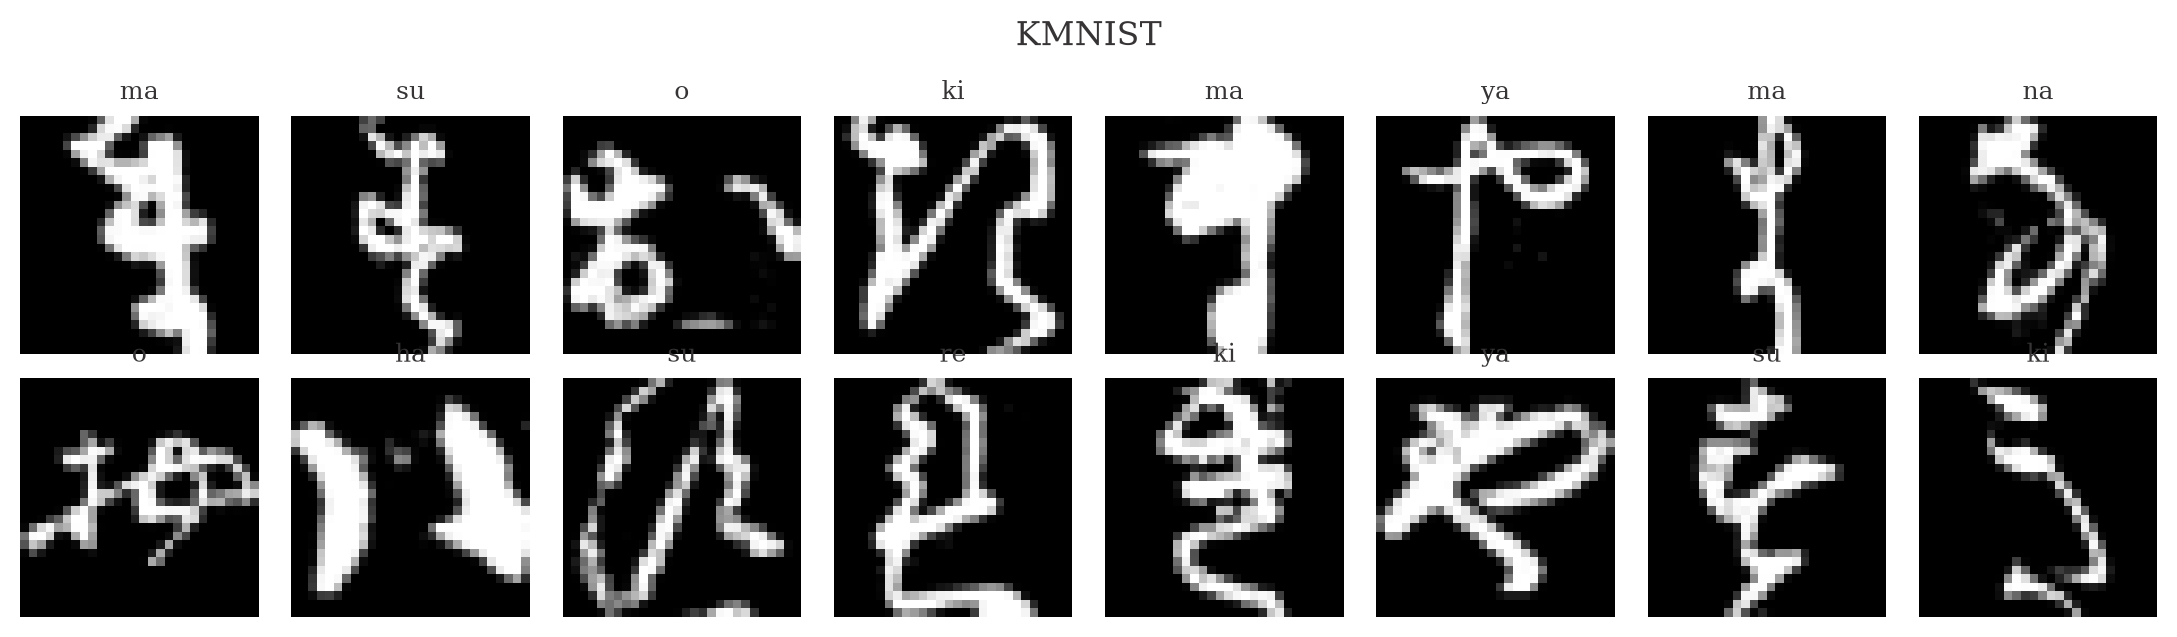
\includegraphics[width=0.52\linewidth]{figuras/f01_muestras.png}\hfill
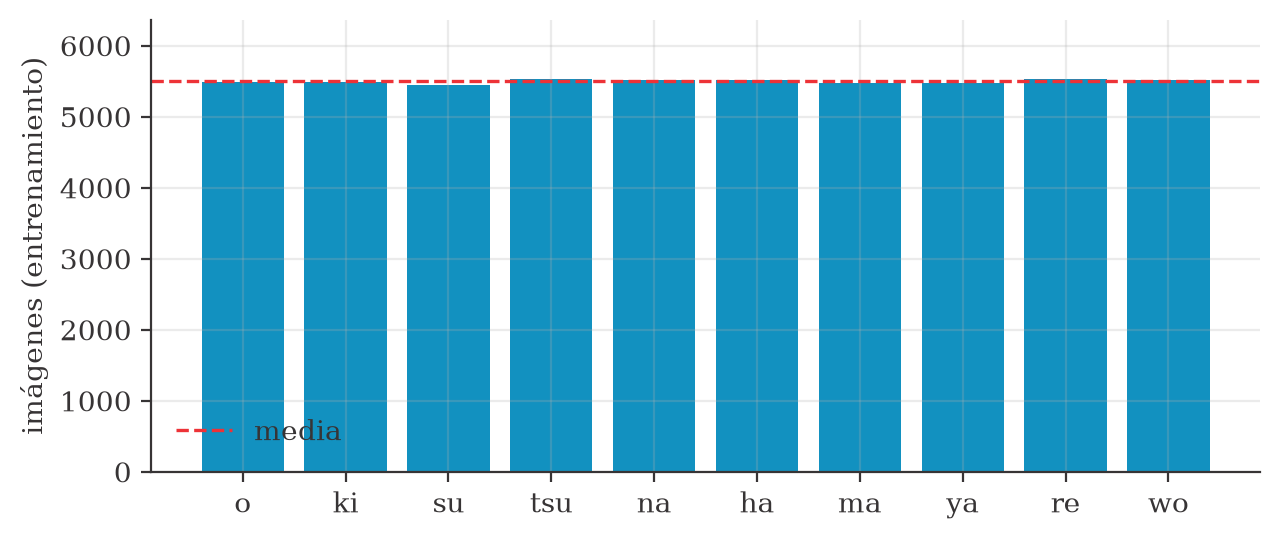
\includegraphics[width=0.44\linewidth]{figuras/f02_conteo_clases.png}
\caption{Muestras de KMNIST (izquierda) y conteo por clase en entrenamiento (derecha).}\label{fig:datos}
\end{figure}

\textbf{Reproducibilidad y comparaciones pareadas.} Toda corrida fija la semilla de Python, NumPy y PyTorch. Se detectó, además,
que el \texttt{DataLoader} de entrenamiento del cuaderno base comparte un único generador entre corridas: su estado avanza, así
que dos entrenamientos con ``la misma semilla'' ven los lotes en órdenes distintos y la comparación no es realmente pareada. En
las comparaciones de este informe se crea un cargador \textbf{nuevo por corrida}, de modo que, dada una semilla, la inicialización,
el orden de los lotes y el \textit{dropout} son idénticos con y sin la modificación evaluada. Los resultados se reportan como media
$\pm$ desviación estándar muestral (ddof\,=\,1) sobre 5 semillas (aumento de datos) o 3 semillas (ablación, líneas base y otros
conjuntos).

%% ---------------------------------------------------------------------------------------------
\section{Arquitectura \texttt{CNNPropia} (TODO 2)}

La red apila dos bloques \texttt{Conv2d(3$\times$3, relleno 1)} $\to$ \texttt{BatchNorm2d} $\to$ ReLU $\to$ \texttt{MaxPool2d(2)}, aplana, aplica
\texttt{Dropout(0,3)} y termina en una capa lineal de 10 \textit{logits}. La función de pérdida es la entropía cruzada (que
incluye la \textit{softmax}), por lo que la red no la aplica por su cuenta.

\begin{table}[!htbp]
\centering\footnotesize
\caption{Arquitectura y parámetros. Total: 20\,586 ($<$ 200\,000, requisito del taller).}
\begin{tabular}{l l r l}
\toprule
Capa & Salida & Parámetros & Cálculo \\
\midrule
Entrada & $1\times28\times28$ & 0 & \\
Conv $3\times3$, 16 filtros, relleno 1 & $16\times28\times28$ & 160 & $16(1\cdot9+1)$ \\
BatchNorm2d(16) & $16\times28\times28$ & 32 & $2\cdot16$ ($\gamma,\beta$) \\
ReLU + MaxPool $2\times2$ & $16\times14\times14$ & 0 & \\
Conv $3\times3$, 32 filtros, relleno 1 & $32\times14\times14$ & 4\,640 & $32(16\cdot9+1)$ \\
BatchNorm2d(32) & $32\times14\times14$ & 64 & $2\cdot32$ \\
ReLU + MaxPool $2\times2$ & $32\times7\times7$ & 0 & \\
Aplanar + Dropout(0,3) & 1\,568 & 0 & $32\cdot7\cdot7$ \\
Lineal $1568\to10$ & 10 & 15\,690 & $1568\cdot10+10$ \\
\bottomrule
\end{tabular}
\end{table}

\textbf{¿Por qué cada componente y qué se esperaba de él?}
\begin{itemize}
  \item \textbf{Convolución $3\times3$}: detecta rasgos locales (bordes, curvas, cruces de trazos) reutilizando los mismos pesos en toda
        la imagen; da pocos parámetros e invarianza parcial a traslaciones. Se esperaba que superara a un MLP con muchos más parámetros
        (confirmado en la sección~\ref{sec:bases}). El relleno 1 conserva el tamaño antes de cada \textit{pooling}.
  \item \textbf{BatchNorm}: se esperaba un entrenamiento más estable y rápido y tolerancia a tasas de aprendizaje mayores. La ablación
        (sección~\ref{sec:abl}) \textbf{no} mostró mejora de exactitud a 5 épocas; el beneficio en estabilidad sí aparece en el barrido de $\eta$
        (sección~\ref{sec:lr}).
  \item \textbf{ReLU}: no linealidad barata que no satura para valores positivos.
  \item \textbf{MaxPool}: divide el tamaño por 2 y da tolerancia a pequeños desplazamientos del trazo.
  \item \textbf{Dropout}: regulariza la capa lineal final, donde está el 76\,\% de los parámetros. La ablación confirma su aporte.
\end{itemize}

%% ---------------------------------------------------------------------------------------------
\section{Entrenamiento (TODO 3)}

Se usa Adam con $\eta = 10^{-3}$, lotes de 64 y \cifraepocas{} épocas. Cada iteración repite, en este orden, los cinco pasos que pide el
taller: \texttt{zero\_grad()} (PyTorch acumula los gradientes y sin borrarlos se mezclan lotes), propagación hacia adelante,
entropía cruzada, \texttt{backward()} (regla de la cadena desde los \textit{logits}, donde $\partial L/\partial z = p - y$) y
\texttt{step()} (Adam actualiza los 20\,586 parámetros a la vez).

\begin{figure}[!htbp]
\centering
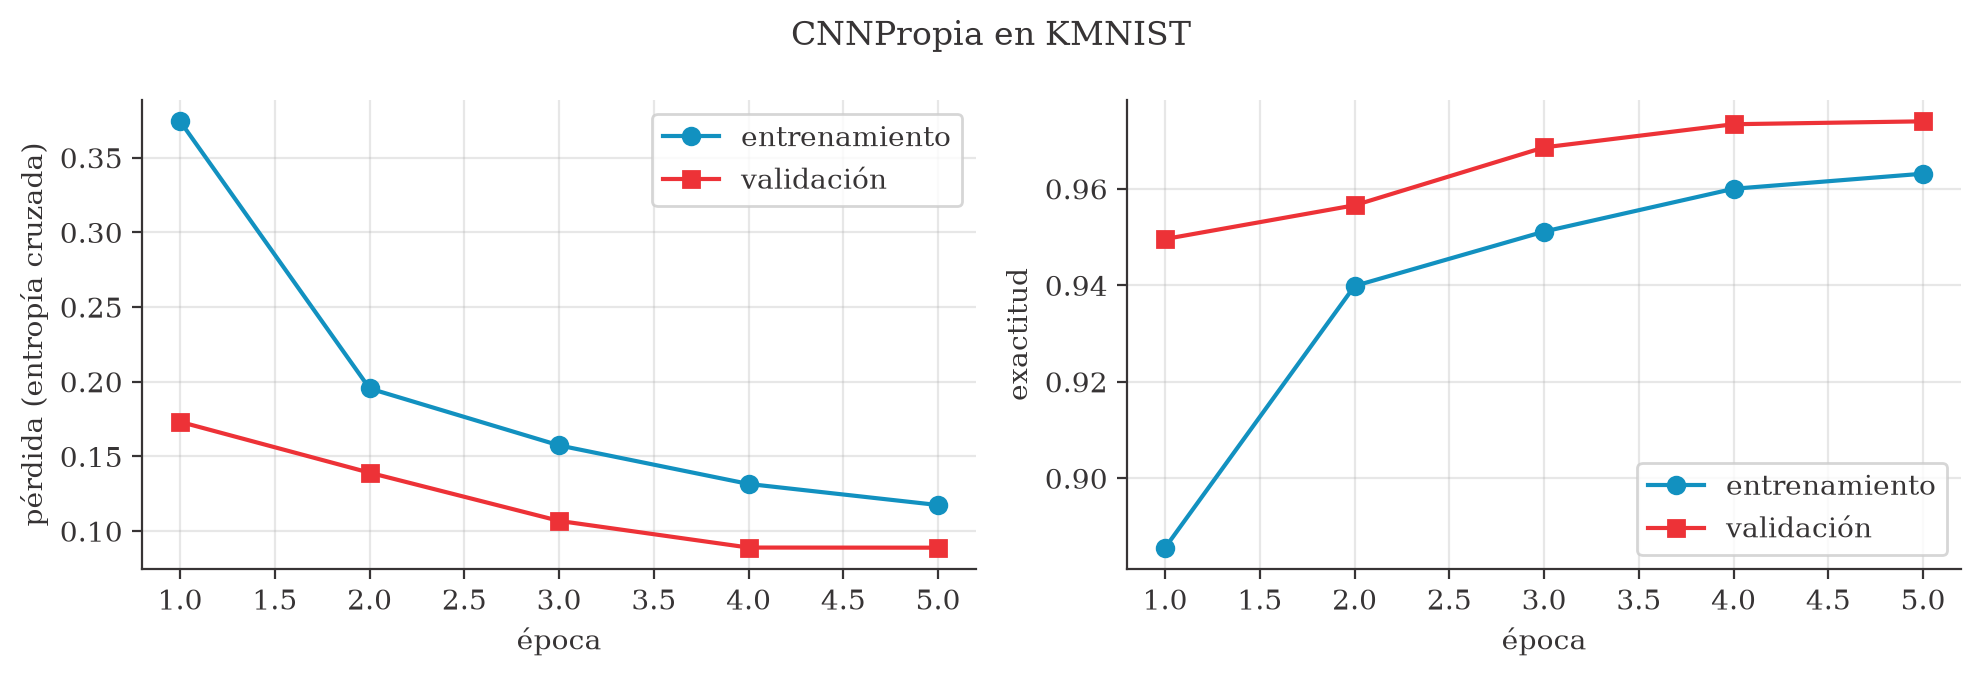
\includegraphics[width=0.92\linewidth]{figuras/f03_curvas_cnnpropia.png}
\caption{Pérdida y exactitud por época. La curva de entrenamiento se promedia durante la época y con \textit{dropout} activo, por lo que
queda por encima de la de validación.}
\end{figure}

\begin{table}[!htbp]
\centering
\caption{Historial del entrenamiento principal.}
\begin{tabular}{lrrrr}
\toprule
Época & Pérdida & Exact. & Pérdida val. & Exact. val. \\
\midrule
1 & 0,3744 & 88,56\,\% & 0,1732 & 94,96\,\% \\
2 & 0,1955 & 93,99\,\% & 0,1391 & 95,66\,\% \\
3 & 0,1574 & 95,11\,\% & 0,1069 & 96,86\,\% \\
4 & 0,1316 & 96,00\,\% & 0,0890 & 97,34\,\% \\
5 & 0,1175 & 96,31\,\% & 0,0889 & 97,40\,\% \\
\bottomrule
\end{tabular}

\end{table}

La pérdida de entrenamiento baja de \cifralossIni{} a \cifralossFin{} y la exactitud de validación llega a \cifraaccVal\,\%. No hay sobreajuste
visible a 5 épocas: la brecha entre exactitud de entrenamiento (en modo evaluación) y validación es de unos 0,9 puntos.

%% ---------------------------------------------------------------------------------------------
\section{Evaluación en prueba y análisis de errores (TODO 4)}

El conjunto de prueba se usó para estimar el rendimiento del modelo final; ninguna decisión de diseño se tomó mirándolo. La exactitud
es \textbf{\cifraaccTest\,\%} (\cifraerrTest{} errores de 10\,000).

\begin{figure}[!htbp]
\centering
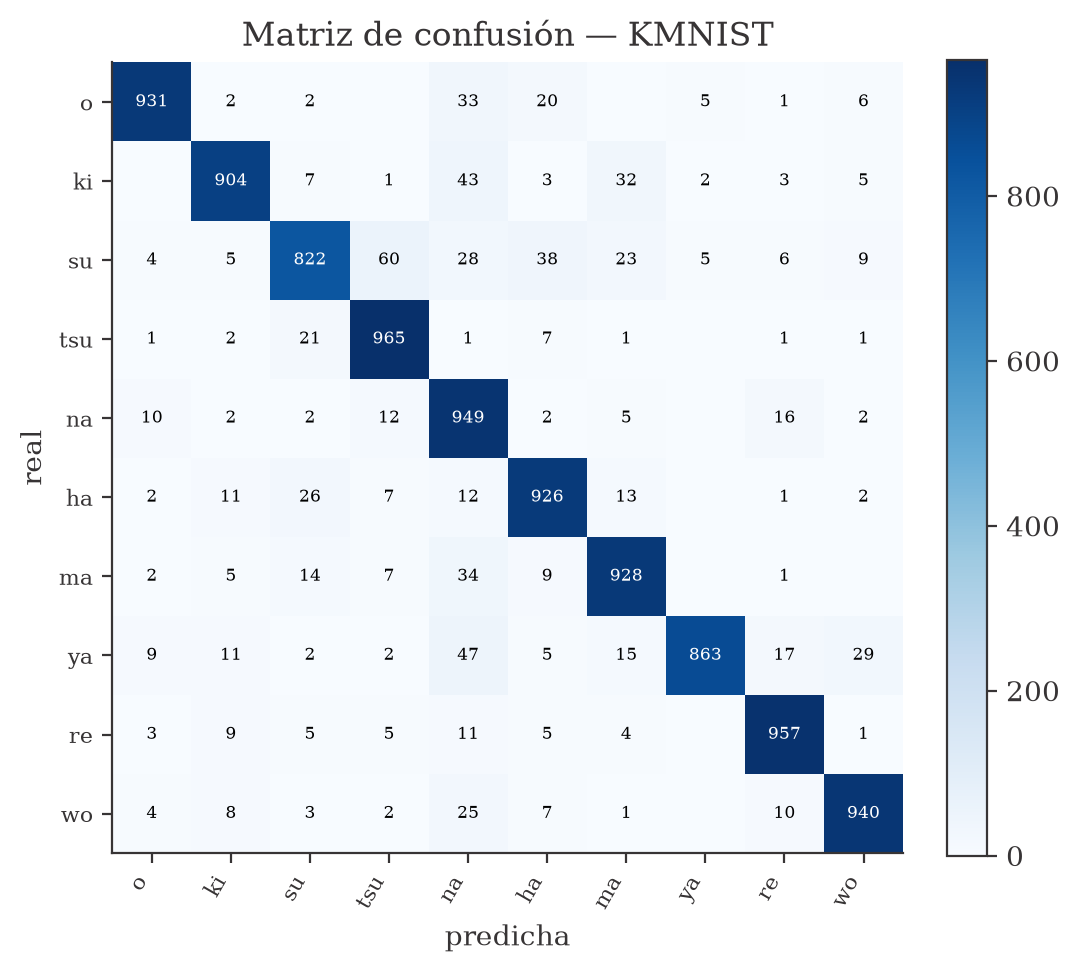
\includegraphics[width=0.48\linewidth]{figuras/f04_matriz_confusion.png}\hfill
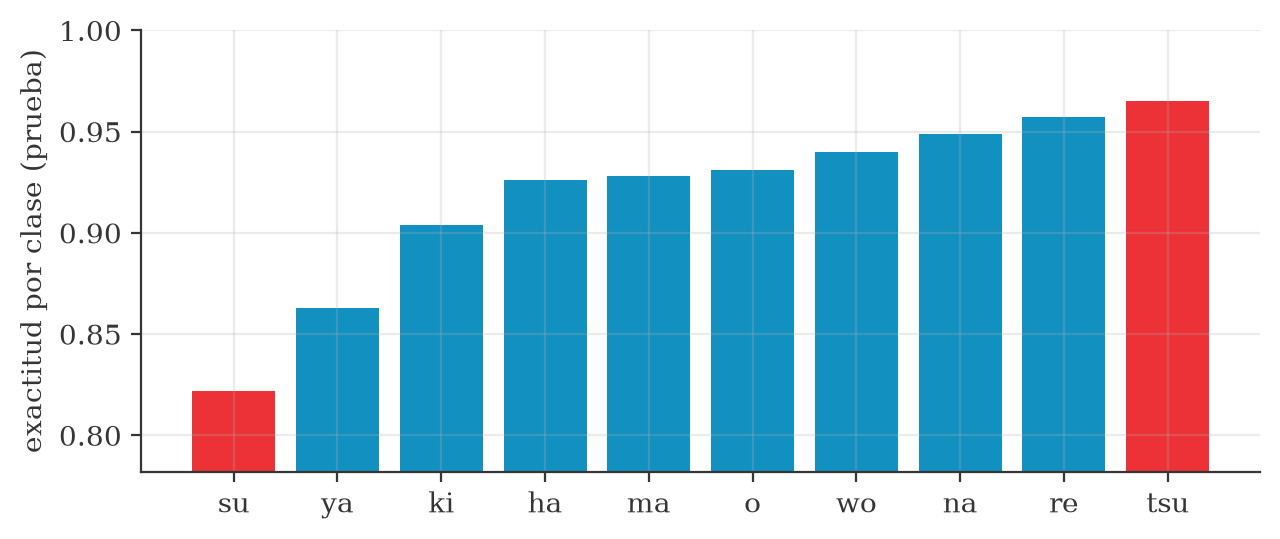
\includegraphics[width=0.48\linewidth]{figuras/f06_acc_por_clase.png}
\caption{Matriz de confusión en prueba y exactitud por clase.}
\end{figure}

\textbf{Brecha entre validación y prueba.} La validación (97,40\,\%) supera a la prueba (\cifraaccTest\,\%) por \cifrabrechaValTest{} puntos. No es un
error del código: se repite con las 5 semillas y \textbf{no aparece} con MNIST ni FashionMNIST (sección~\ref{sec:datasets}). La validación
sale de una partición aleatoria del entrenamiento y comparte su distribución; la prueba oficial de KMNIST no la comparte del todo. La causa exacta
no se midió; una hipótesis razonable es que haya variantes de escritura o escritores presentes solo en prueba. Para reportar rendimiento hay que mirar la
prueba; la validación sirve para \textit{comparar} configuraciones, no para predecir el número final.

\textbf{Par más confundido.}
\begin{table}[!htbp]
\centering
\caption{Cinco pares (real $\to$ predicha) con más errores en prueba.}
\begin{tabular}{lrr}
\toprule
Real $\to$ predicha & Veces & Sentido contrario \\
\midrule
su $\to$ tsu & 60 & 21 \\
ya $\to$ na & 47 & 0 \\
ki $\to$ na & 43 & 2 \\
su $\to$ ha & 38 & 26 \\
ma $\to$ na & 34 & 5 \\
\bottomrule
\end{tabular}

\end{table}

El par más frecuente es \textbf{\cifraparA{} $\to$ \cifraparB{}} (\cifraparN{} veces; en sentido contrario, \cifraparInv). \textit{su} es además la clase más difícil
(\cifraclasePeorAcc\,\%) y \textit{\cifraclaseMejor} la más fácil (\cifraclaseMejorAcc\,\%). Al mirar imágenes concretas (figura~\ref{fig:par}), los \textit{su} mal
clasificados son casi siempre una \textbf{variante cursiva} distinta de la dominante en la clase (trazo vertical largo con ganchos a la derecha, sin el bucle
característico de la forma estándar), parecida a varias grafías de \textit{tsu} bien clasificadas. Es \textbf{variación dentro de la clase}: el kuzushiji conserva formas
alternativas del mismo carácter. Que la confusión sea asimétrica (60 frente a 21) sugiere que \textit{tsu} actúa como ``atractor'' de esas variantes raras de
\textit{su}. Algo similar ocurre con \textit{na}, clase predicha en tres de los cinco pares más frecuentes y casi nunca confundida en sentido inverso.

\begin{figure}[!htbp]
\centering
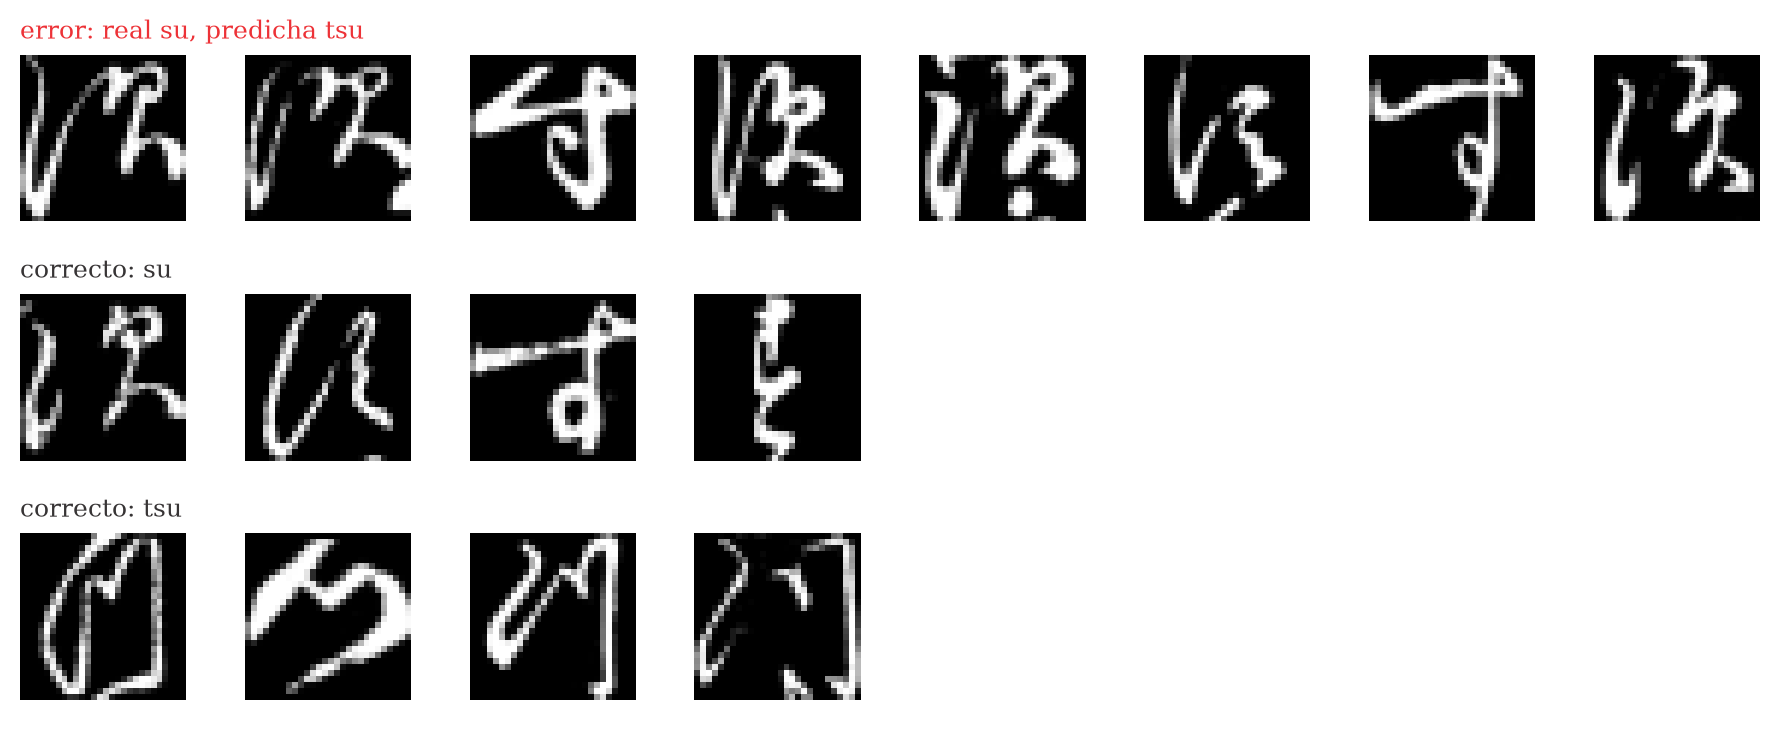
\includegraphics[width=0.9\linewidth]{figuras/f05_par_confundido.png}
\caption{Arriba, errores \textit{su} leído como \textit{tsu}; abajo, aciertos de cada clase para contraste.}\label{fig:par}
\end{figure}

%% ---------------------------------------------------------------------------------------------
\section{Aumento de datos (TODO 5)}

Se implementó un desplazamiento aleatorio de hasta $\pm2$ píxeles con \texttt{torch.roll}: uno por lote (el del taller) y, como extra, uno distinto por imagen.
Se comparó con y sin aumento con 5 semillas pareadas (tabla~\ref{tab:aug}).

\begin{table}[!htbp]
\centering
\caption{Aumento de datos, 5 épocas, 5 semillas. ``Entren. (eval)'' es la exactitud de entrenamiento con el modelo en modo evaluación; la brecha es
entren.\,$-$\,validación.}\label{tab:aug}
\footnotesize
\begin{tabular}{lrrrrr}
\toprule
Configuración & $n$ & Entren. (eval) & Validación (\%) & Prueba (\%) & Brecha \\
\midrule
sin aumento & 5 & 98,00\,\% & 97,10 $\pm$ 0,27 & 92,13 $\pm$ 0,28 & 0,90\,pts \\
con aumento (lote) & 5 & 97,30\,\% & 97,09 $\pm$ 0,13 & 91,81 $\pm$ 0,15 & 0,21\,pts \\
con aumento (por muestra) & 5 & 97,43\,\% & 97,22 $\pm$ 0,13 & 91,89 $\pm$ 0,24 & 0,22\,pts \\
\bottomrule
\end{tabular}

\end{table}

\textbf{¿Mejoró la exactitud de validación?} No. Frente a ``sin aumento'': por lote \cifraaugLoteVal\pts{} en validación y \cifraaugLoteTe\pts{} en prueba (mejor en
\cifraaugLoteTeGana{} de \cifraaugN{} semillas); por muestra \cifraaugMuestraVal\pts{} en validación y \cifraaugMuestraTe\pts{} en prueba. Las diferencias están dentro del ruido
entre semillas (0,3 a 0,4 puntos).

\textbf{¿Cambió la brecha entre entrenamiento y validación?} Sí: baja de 0,90 puntos a unos 0,2. El aumento regulariza (la red memoriza menos), pero esa menor memorización
no se traduce en mejor generalización. Posibles razones, hipótesis no probadas por separado: (a) con 5 épocas casi no hay sobreajuste que corregir; (b) convolución más
\textit{max-pooling} ya tolera desplazamientos pequeños; (c) \texttt{torch.roll} es circular y reinserta por el borde opuesto lo que sale; (d) los errores en prueba parecen
venir de variantes de escritura, no de traslaciones.

\textbf{¿Y con más épocas?} Con 15 épocas (3 semillas) el modelo sin aumento sí empieza a memorizar y el aumento recorta esa brecha (de \cifralargoBrechaSin\pts{} a \cifralargoBrechaCon\pts{}),
pero otra vez sin mejorar: \cifralargoValDif\pts{} en validación y \cifralargoTeDif\pts{} en prueba.

\begin{table}[!htbp]
\centering
\caption{Aumento por muestra con 15 épocas, 3 semillas.}
\footnotesize
\begin{tabular}{lrrrrr}
\toprule
Configuración (15 épocas) & $n$ & Entren. (eval) & Validación (\%) & Prueba (\%) & Brecha \\
\midrule
sin aumento & 3 & 99,32\,\% & 98,23 $\pm$ 0,18 & 94,15 $\pm$ 0,18 & 1,09\,pts \\
con aumento (por muestra) & 3 & 98,48\,\% & 98,08 $\pm$ 0,18 & 93,96 $\pm$ 0,14 & 0,40\,pts \\
\bottomrule
\end{tabular}

\end{table}

\begin{figure}[!htbp]
\centering
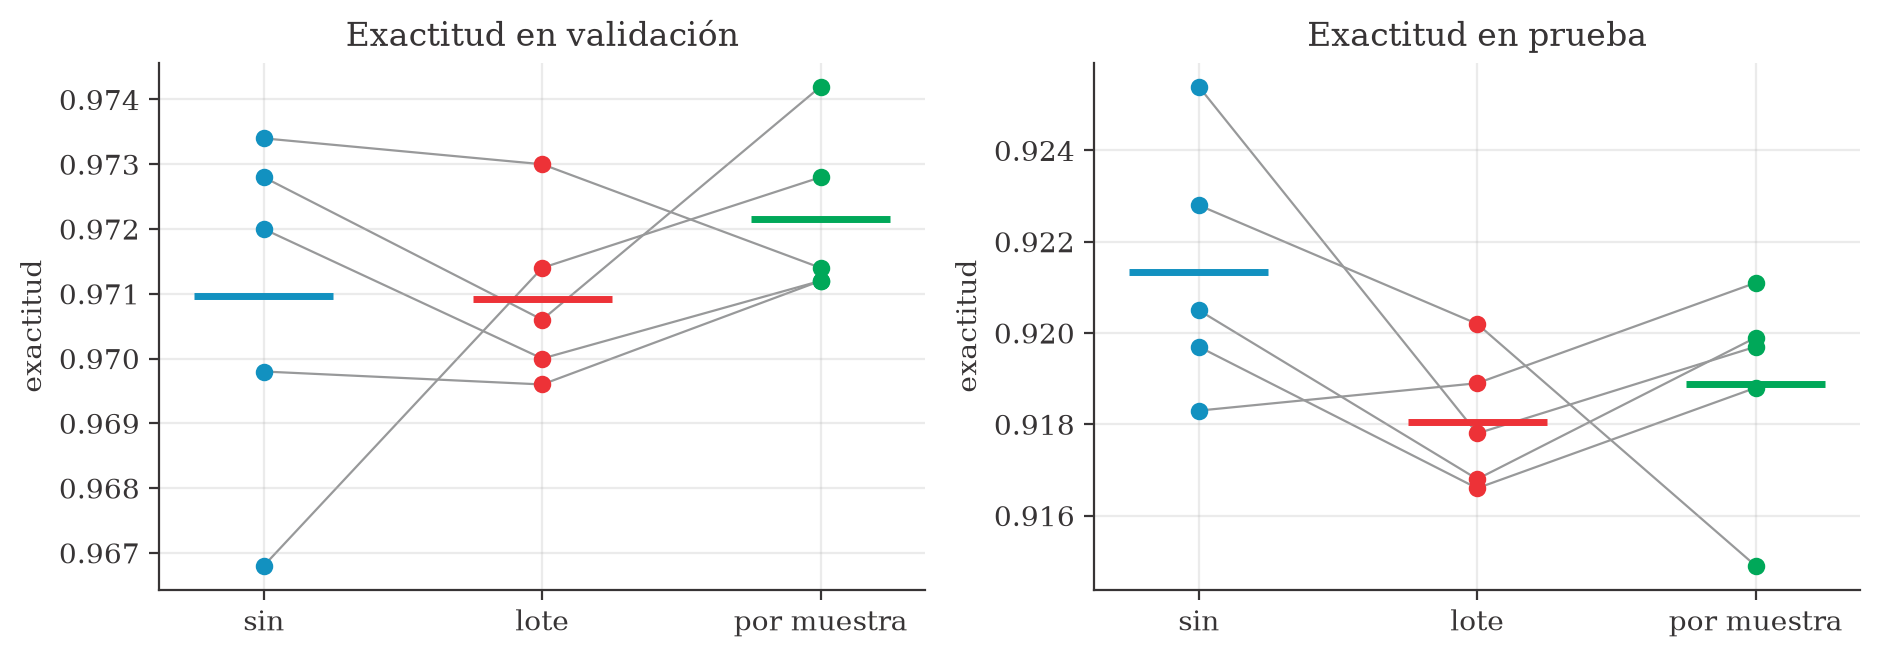
\includegraphics[width=0.98\linewidth]{figuras/f08_aumento_semillas.png}
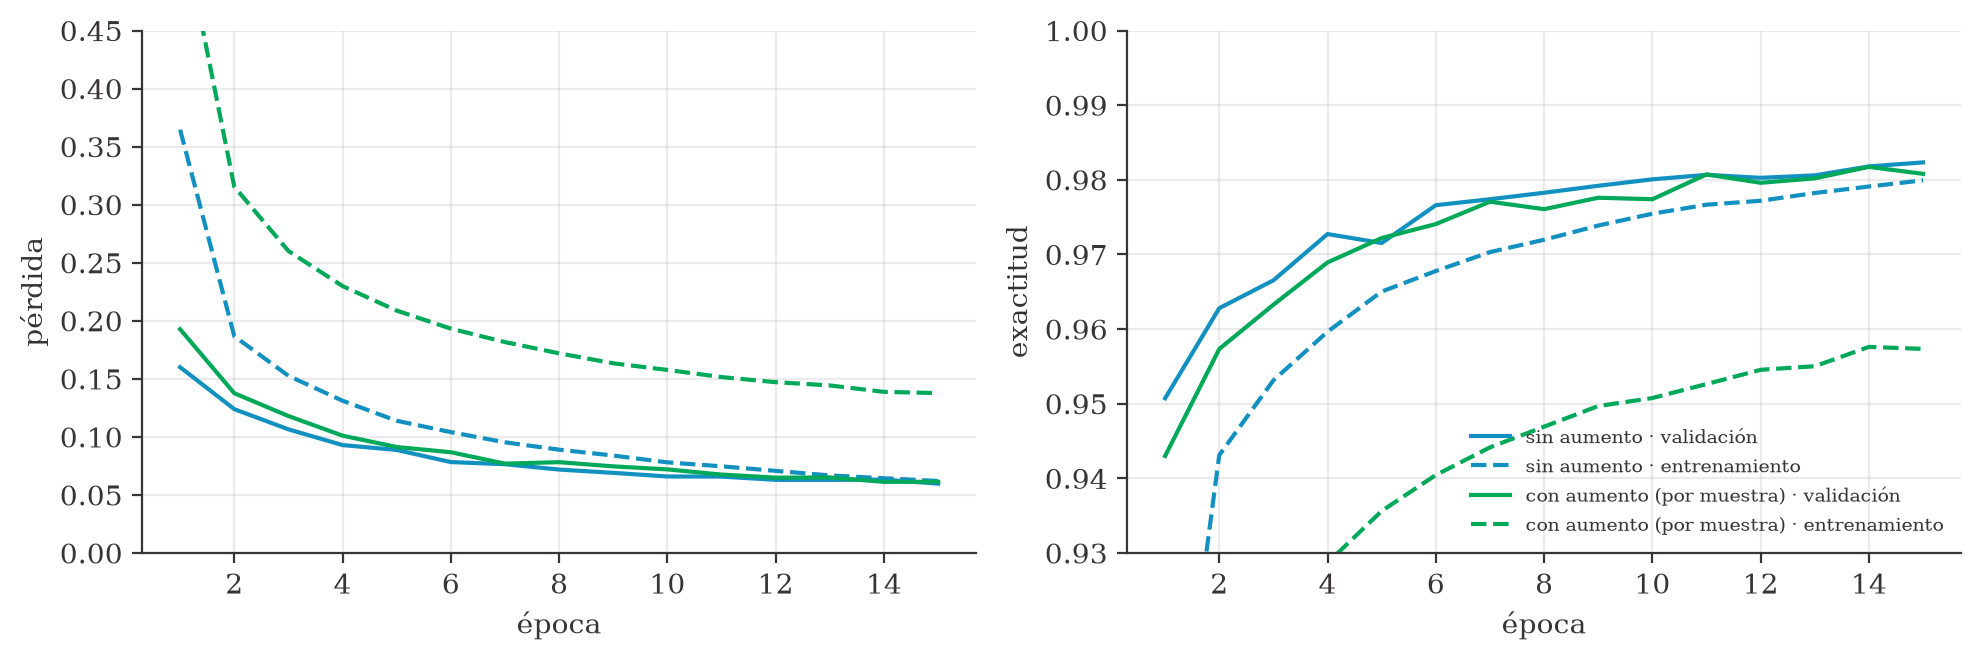
\includegraphics[width=0.98\linewidth]{figuras/f08b_aumento_15_epocas.png}
\caption{Arriba: una semilla por punto (las líneas grises unen la misma semilla). Abajo: curvas medias con 15 épocas.}
\end{figure}

%% ---------------------------------------------------------------------------------------------
\section{Extras}

\subsection{Ablación de componentes y profundidad}\label{sec:abl}
Se quita una pieza a la vez, con 3 semillas pareadas.

\begin{table}[!htbp]
\centering
\caption{Ablación, 5 épocas, 3 semillas.}
\footnotesize
\begin{tabular}{lrrrrr}
\toprule
Variante & Parám. & Entren. (eval) & Validación (\%) & Prueba (\%) & Brecha \\
\midrule
completa (16-32, BN, Dropout) & 20\,586 & 98,06\,\% & 97,15 $\pm$ 0,16 & 92,10 $\pm$ 0,16 & 0,90\,pts \\
sin BatchNorm & 20\,490 & 98,30\,\% & 97,47 $\pm$ 0,25 & 92,64 $\pm$ 0,34 & 0,83\,pts \\
sin Dropout & 20\,586 & 98,14\,\% & 96,69 $\pm$ 0,20 & 91,58 $\pm$ 0,35 & 1,45\,pts \\
sin BatchNorm ni Dropout & 20\,490 & 98,72\,\% & 97,26 $\pm$ 0,09 & 92,56 $\pm$ 0,51 & 1,46\,pts \\
3 bloques (16-32-64) & 29\,290 & 99,12\,\% & 98,23 $\pm$ 0,16 & 94,21 $\pm$ 0,29 & 0,89\,pts \\
\bottomrule
\end{tabular}

\end{table}

\begin{itemize}
  \item \textbf{Dropout aporta}: quitarlo baja la validación \cifraablDropVal\pts{} y la prueba \cifraablDropTe\pts{}, y sube la brecha a \cifraablDropBrecha\pts{} (frente a \cifraablBrechaCompleta).
  \item \textbf{BatchNorm no mejoró la exactitud} a 5 épocas con $\eta = 10^{-3}$: sin ella la validación cambia \cifraablBnVal\pts{} y la prueba \cifraablBnTe\pts{} (con 3 semillas es
        indistinguible del ruido). Esto contradice la expectativa de ``estabiliza y acelera'' en cuanto a la \textit{exactitud} y se anota como tal.
  \item \textbf{El tercer bloque es la mejora clara}: \cifraablTresVal\pts{} en validación y \cifraablTresTe\pts{} en prueba con 8\,704 parámetros más (+42\,\%). La brecha no cambia, es decir, la red base
        estaba \textbf{subajustada}; faltaba capacidad y campo receptivo, no regularización.
\end{itemize}
\begin{center}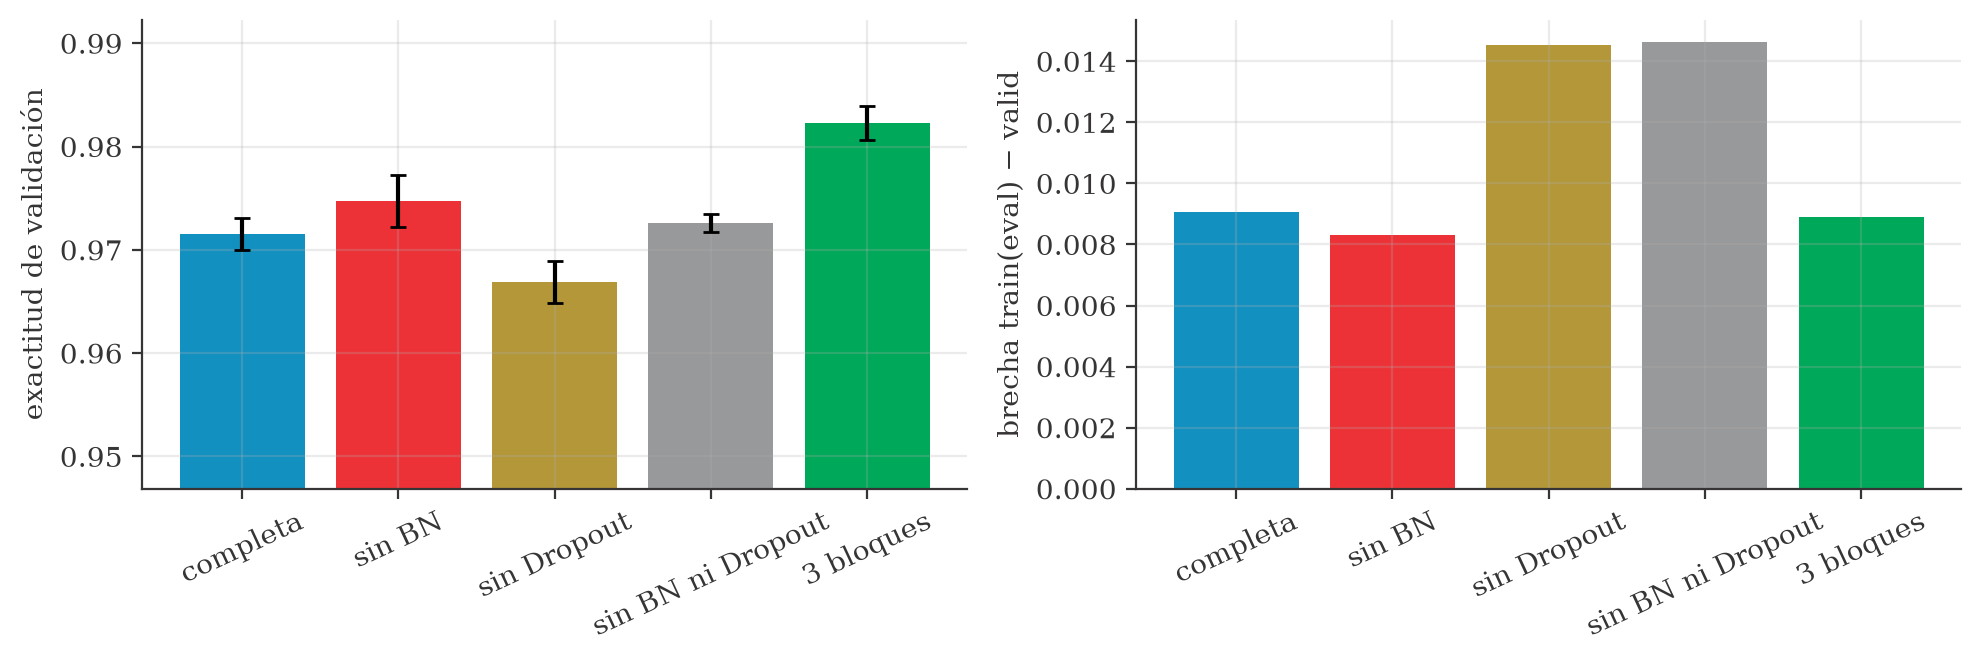
\includegraphics[width=0.95\linewidth]{figuras/f09_ablacion.png}\end{center}

\subsection{Líneas base: MLP y CNN del docente}\label{sec:bases}
\begin{table}[!htbp]
\centering
\caption{Mismas condiciones sobre KMNIST, 3 semillas. Tiempos en CPU.}
\footnotesize
\begin{tabular}{lrrrr}
\toprule
Modelo & Parám. & Validación (\%) & Prueba (\%) & Tiempo \\
\midrule
MLP docente (784-128-10) & 101\,770 & 95,45 $\pm$ 0,18 & 88,44 $\pm$ 0,59 & 3\,s \\
CNN docente (12 810 par.) & 12\,810 & 96,87 $\pm$ 0,04 & 91,20 $\pm$ 0,37 & 36\,s \\
CNNPropia (20 586 par.) & 20\,586 & 97,15 $\pm$ 0,16 & 92,10 $\pm$ 0,16 & 48\,s \\
\bottomrule
\end{tabular}

\end{table}

La CNN pequeña del docente (12\,810 parámetros) supera al MLP (101\,770) y generaliza mejor; \texttt{CNNPropia} gana \cifracnnPropVsDoc\pts{} adicionales sobre esa CNN y
\cifracnnPropVsMlp\pts{} sobre el MLP (prueba: \cifracnnPropTe\,\% frente a \ciframlpTe\,\%). El MLP memoriza (brecha de 3,1 puntos).

\subsection{KMNIST frente a MNIST y FashionMNIST}\label{sec:datasets}
\begin{table}[!htbp]
\centering
\caption{La misma \texttt{CNNPropia}, sin cambios, en tres conjuntos (3 semillas).}
\footnotesize
\begin{tabular}{lrrrrr}
\toprule
Dataset & Validación (\%) & Prueba (\%) & Val.$-$prueba & Peor clase & Clases $<$ 90\,\% \\
\midrule
MNIST & 98,72 $\pm$ 0,09 & 98,80 $\pm$ 0,18 & $-$0,1\,pts & 97,2\,\% & 0,0 \\
FashionMNIST & 90,34 $\pm$ 0,45 & 90,27 $\pm$ 0,10 & 0,1\,pts & 72,2\,\% & 4,3 \\
KMNIST & 97,15 $\pm$ 0,16 & 92,10 $\pm$ 0,16 & 5,1\,pts & 86,3\,\% & 2,0 \\
\bottomrule
\end{tabular}

\end{table}

Por exactitud en prueba, KMNIST (\cifradsKMNISTTe\,\%) es más difícil que MNIST (\cifradsMNISTTe\,\%) y algo más fácil que FashionMNIST (\cifradsFashionMNISTTe\,\%); por peor clase, KMNIST queda entre ambos.
Lo distintivo de KMNIST es su \textbf{brecha validación--prueba} (\cifradsKMNISTGap\,pts frente a $\approx 0$ en los otros dos).

\subsection{Tasa de aprendizaje}\label{sec:lr}
\begin{table}[!htbp]
\centering
\caption{Barrido de $\eta$ con Adam, 2 épocas, una semilla (exploratorio), con BatchNorm y sin ella (control).}
\footnotesize
\begin{tabular}{lrrr}
\toprule
$\eta$ & Val. con BN & Val. sin BN & Pérdida val. (con BN) \\
\midrule
$10^{-1}$ & 82,46\,\% & 9,76\,\% & 0,584 \\
$10^{-2}$ & 96,70\,\% & 92,62\,\% & 0,107 \\
$10^{-3}$ & 96,30\,\% & 96,52\,\% & 0,128 \\
$10^{-4}$ & 92,38\,\% & --- & 0,265 \\
$10^{-5}$ & 76,30\,\% & --- & 0,968 \\
\bottomrule
\end{tabular}

\end{table}

El óptimo está entre $10^{-2}$ (\cifralrDos\,\%) y $10^{-3}$ (\cifralrTres\,\%); la diferencia no es concluyente con una semilla. La CNN del docente (sin BatchNorm) se quedó en $\approx 10$\,\% en MNIST con $\eta = 10^{-1}$, pero ese resultado mezcla red y conjunto. Por eso se hizo un \textbf{control}: la misma \texttt{CNNPropia} sin BatchNorm.
Con $\eta = 10^{-1}$ cae a \cifralrSinBnUno\,\% (no aprende, igual que en el script del docente) mientras que con BatchNorm llega a \cifralrUno\,\%; con $10^{-2}$ la diferencia es \cifralrDos\,\% frente a \cifralrSinBnDos\,\%, y con $10^{-3}$ es nula (\cifralrTres\,\% frente a \cifralrSinBnTres\,\%).
Es decir, \textbf{BatchNorm no mejora la exactitud con una $\eta$ bien elegida, pero ensancha el rango de $\eta$ que funciona}. Es una sola semilla, pero a $10^{-1}$ la diferencia es de unos 73 puntos.

\subsection{Lo que aprende la red}
Los filtros de la primera capa se mueven (en promedio cambian 46\,\% de su norma respecto a la inicialización), pero con 9 pesos por filtro y 5 épocas no se ven como detectores de bordes
``de libro'' y no conviene forzar esa interpretación. Los mapas del bloque 1 se encienden sobre los trazos; los del bloque 2 son más dispersos y responden a fragmentos de trazo.

\begin{figure}[!htbp]
\centering
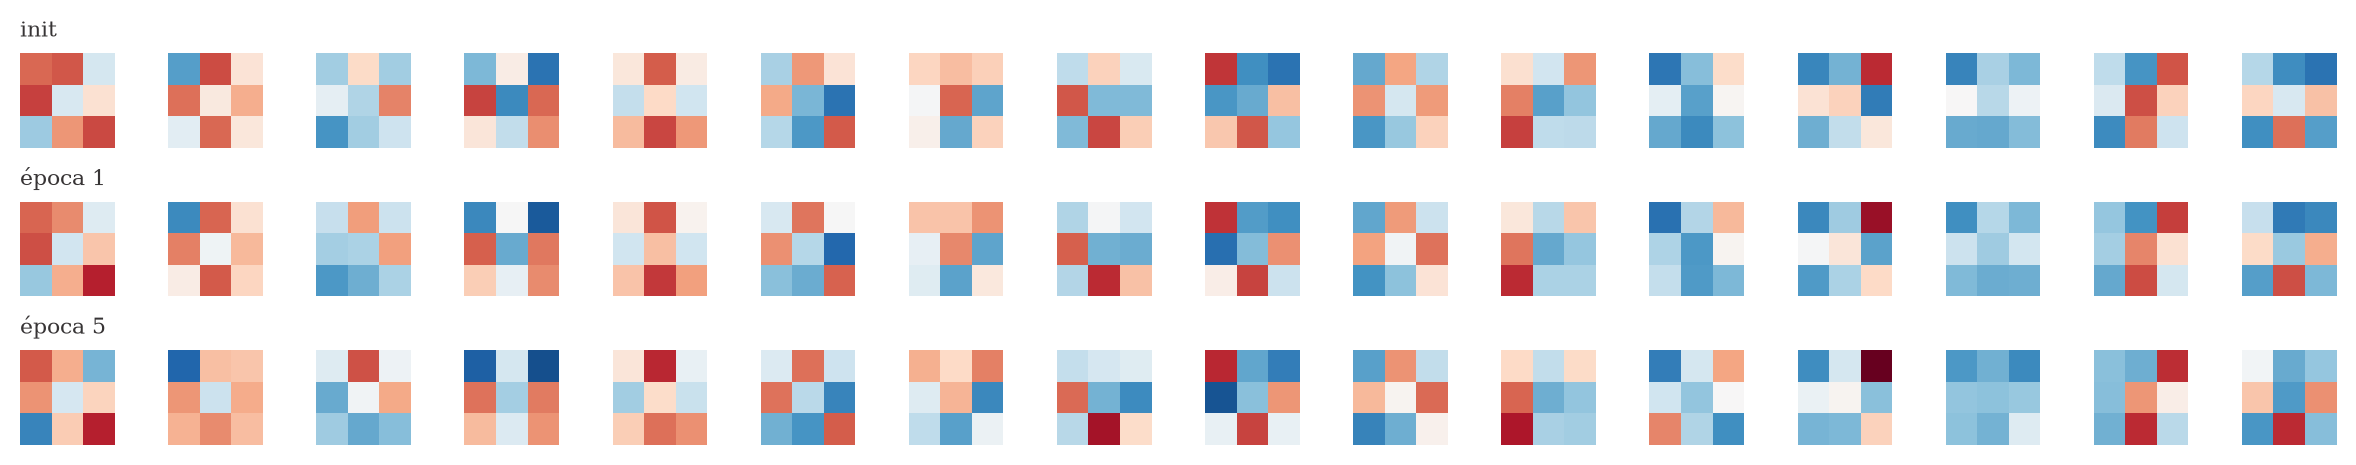
\includegraphics[width=0.98\linewidth]{figuras/f13_filtros_conv1.png}
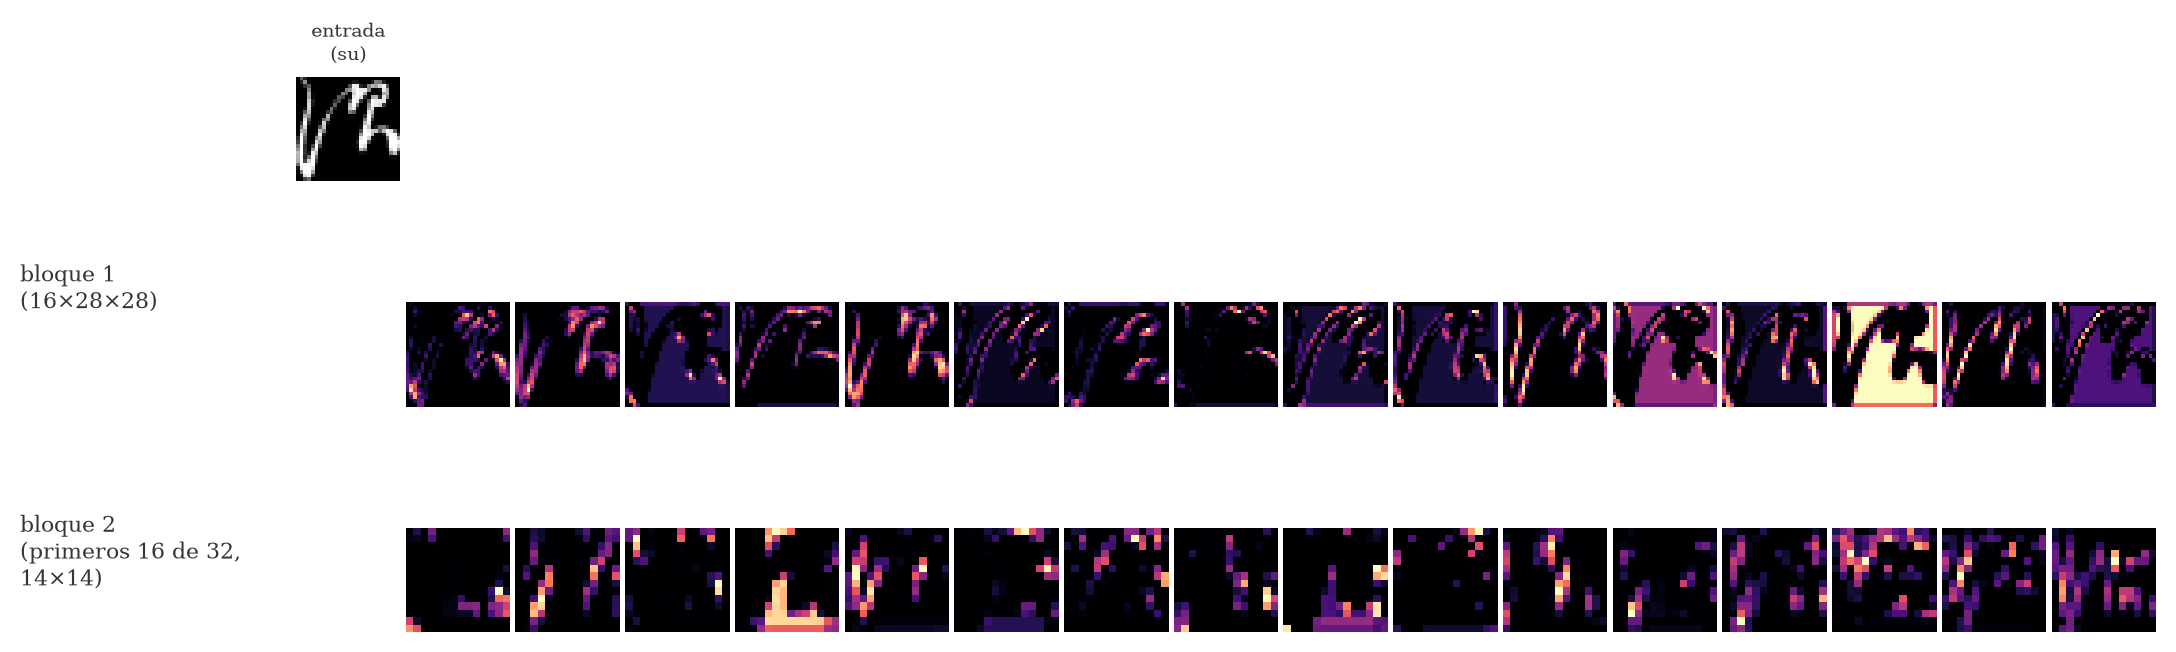
\includegraphics[width=0.98\linewidth]{figuras/f14_mapas_activacion.png}
\caption{Filtros de la primera capa (inicio, época 1, época 5) y mapas de activación de ambos bloques para un carácter de prueba.}
\end{figure}

%% ---------------------------------------------------------------------------------------------
\section{Discusión y limitaciones}

\begin{itemize}
  \item \textbf{Validación y prueba no son intercambiables en KMNIST.} Con la validación aleatoria se habría reportado $\approx 97$\,\%; el rendimiento esperado en prueba es $\approx 92$\,\%.
  \item \textbf{Lo que falla es variación intra-clase.} Los errores se concentran en variantes cursivas de un mismo carácter; más épocas o más regularización no atacan eso. Un tercer bloque (+2,1 pts) sí ayuda.
  \item \textbf{Un resultado nulo es un resultado.} El aumento por desplazamiento regularizó pero no mejoró; ensayar rotaciones pequeñas o deformaciones elásticas queda como trabajo futuro.
  \item \textbf{Alcance.} 3 a 5 semillas, 5 épocas (15 en el extra del aumento), una arquitectura base y una partición de validación fija: las diferencias de décimas de punto no son concluyentes.
  \item \textbf{Cómo se eligió $\eta$.} Se usó $10^{-3}$ por el enunciado; el barrido sugiere que $10^{-2}$ habría sido igual o ligeramente mejor.
\end{itemize}

%% ---------------------------------------------------------------------------------------------
\section{Conclusiones}

\begin{enumerate}
  \item El taller se resolvió completo: los cinco TODO pasan sus verificaciones. \texttt{CNNPropia} (20\,586 parámetros) logra \cifraaccVal\,\% en validación y \cifraaccTest\,\% en prueba.
  \item En KMNIST el número que importa es el de prueba, unos \cifrabrechaValTest{} puntos por debajo del de validación; es una propiedad del conjunto, no un fallo.
  \item Los errores se explican por variantes cursivas de un mismo carácter (\textit{su}$\to$\textit{tsu}, y varias clases $\to$ \textit{na}), no por desbalance.
  \item El aumento por desplazamiento no mejoró la exactitud ni a 5 ni a 15 épocas, aunque redujo la memorización.
  \item Dropout y más profundidad sí funcionaron; la red base estaba subajustada. Una CNN pequeña supera claramente al MLP con una fracción de los parámetros.
  \item Se comparó siempre con semillas pareadas y se reportaron los resultados negativos tal cual.
\end{enumerate}

\section*{Reproducibilidad}
Todo el código está en \texttt{desarrollo/} (\texttt{build\_notebook.py} genera el cuaderno \texttt{Taller\_3\_CNN\_KMNIST\allowbreak.ipynb}); \texttt{make notebook} lo ejecuta completo (aprox. 1\,h en CPU; las corridas
costosas se guardan en \texttt{resultados/\allowbreak corridas.jsonl}) y \texttt{make rapido} ejecuta solo el núcleo. Versiones: Python 3.12, PyTorch 2.14.1, torchvision 0.29.1. Semillas
de las comparaciones: 0--4 (aumento) y 0--2 (ablación, bases, conjuntos); partición con semilla 42. La animación interactiva está en \texttt{animacion/index.html}.

\begin{thebibliography}{9}
\small
\bibitem{clanuwat} T.~Clanuwat \textit{et al.}, ``Deep Learning for Classical Japanese Literature,'' arXiv:1812.01718, 2018.
\bibitem{lecun} Y.~LeCun, L.~Bottou, Y.~Bengio y P.~Haffner, ``Gradient-based learning applied to document recognition,'' \textit{Proc. IEEE}, 86(11), 1998.
\bibitem{xiao} H.~Xiao, K.~Rasul y R.~Vollgraf, ``Fashion-MNIST: a novel image dataset for benchmarking machine learning algorithms,'' arXiv:1708.07747, 2017.
\bibitem{ioffe} S.~Ioffe y C.~Szegedy, ``Batch Normalization: accelerating deep network training by reducing internal covariate shift,'' \textit{ICML}, 2015.
\bibitem{srivastava} N.~Srivastava \textit{et al.}, ``Dropout: a simple way to prevent neural networks from overfitting,'' \textit{JMLR}, 15, 2014.
\bibitem{kingma} D.~P.~Kingma y J.~Ba, ``Adam: a method for stochastic optimization,'' \textit{ICLR}, 2015.
\bibitem{paszke} A.~Paszke \textit{et al.}, ``PyTorch: an imperative style, high-performance deep learning library,'' \textit{NeurIPS}, 2019.
\end{thebibliography}

\end{document}
